\title{Advanced Topics in Programming Language - Duck Typing in Python}
\author{
        Tommaso Puccetti \\
                Studente presso Universita degli studi di Firenze
}
\date{\today}
\documentclass[12pt]{article}
\usepackage[english]{babel}
\usepackage{graphicx}
\usepackage{hyperref}
\usepackage[procnames]{listings}
\usepackage{jlcode}
\usepackage{color}


\definecolor{keywords}{RGB}{255,0,90}
\definecolor{comments}{RGB}{0,0,113}
\definecolor{red}{RGB}{160,0,0}
\definecolor{green}{RGB}{0,150,0}

\lstset{language=Python, 
	backgroundcolor=\color{white},
	basicstyle=\ttfamily\small, 
	keywordstyle=\color{keywords},
	commentstyle=\color{comments},
	stringstyle=\color{green},
	showstringspaces=false,
	identifierstyle=\color{black},
	procnamekeys={def,class},
}
	

\begin{document}
\maketitle
\tableofcontents
\listoftables
\listoffigures

\section{Possible references}
	\begin{itemize}
		\item \href{https://www.youtube.com/watch?v=fK5lcaNqdj4}{You Tube video};
		\item \href{https://hackernoon.com/python-duck-typing-or-automatic-interfaces-73988ec9037f}{Python duck typing (or automatic interfaces)- how change the dependecy injection};
		\item \href{https://medium.com/programming-hacks/duck-typing-in-python-6740aa72b301}{Simple example};
		\item \href{http://www.voidspace.org.uk/python/articles/duck_typing.shtml}{Something more technical};
		\item 
		\href{https://realpython.com/python-type-checking/}{Ultimate guide to Python's type checking;}
		\item
		\href{https://stackoverflow.com/questions/1517582/what-is-the-difference-between-statically-typed-and-dynamically-typed-languages}{Static vs Dynamic (Stack Overflow)}
		\item
		\href{https://wiki.python.org/moin/Why is Python a dynamic language and also a strongly typed language}{Why Python is dynamic and strongly typed}
		\item
		\href{https://android.jlelse.eu/magic-lies-here-statically-typed-vs-dynamically-typed-languages-d151c7f95e2b}{Maybe schematic overview on typechecking}
		\item
		\href{https://stackoverflow.com/questions/972/adding-a-method-to-an-existing-object-instance}{Bound methods vs Function}
		\item
		\href{https://stackoverflow.com/questions/41692473/does-python-type-hint-annotations-cause-some-run-time-effects}{Annotation power in Python}
		\href{https://stackoverflow.com/questions/972/adding-a-method-to-an-existing-object-instance}{Adding a method to a class}
	\end{itemize}

\section{Questions}
	\begin{itemize}
		\item Are language that implement type inference always static ?
	\end{itemize}
\newpage
\section{Type checking: classification}
	\textbf{Type checking} is the process of verifying and enforces the typing rules of a language. In other words the \textbf{type checker} (the type checking algorithm of the language ) is used to prove the \textbf{type safety} of a program.\\
	Here the possible categories:
	\begin{itemize}
		\item Dynamic vs. Static;
		\item Explicit vs Implicit;
		\item Weakly vs Strongly
	\end{itemize}

	\begin{figure}[h!]
		\centering
		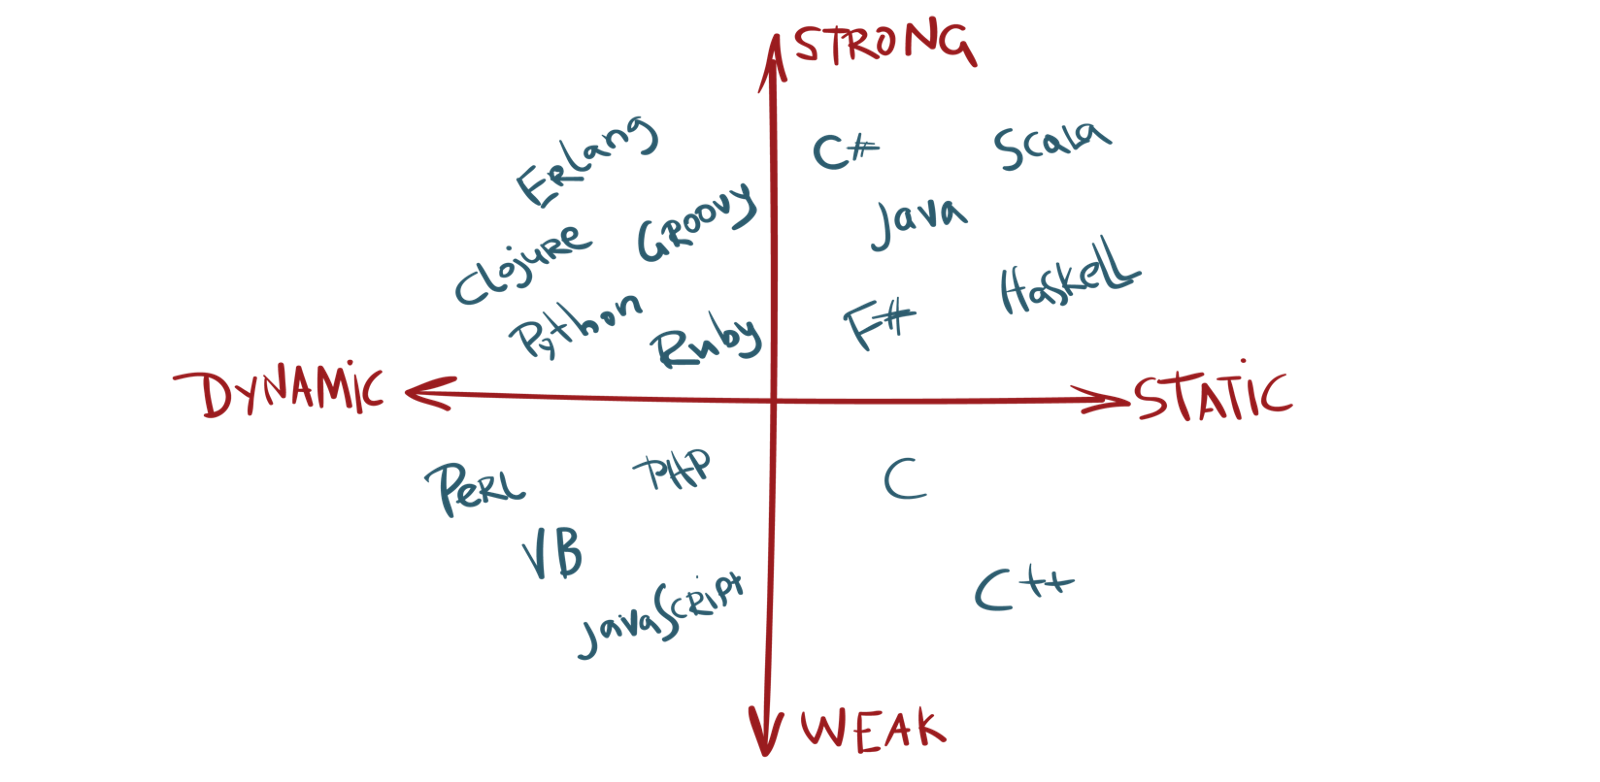
\includegraphics[scale=0.20]{img/classification.png}
	\end{figure}

	\subsection{Static type checking}
		Is the process of verifying the type safety of a program based on the analysis of a program text.  If a program passes a static type checker, then the program is guaranteed to satisfy some set of type safety properties for all possible inputs \textit{\textbf{(Wikipedia)}}.\\
		A language is statically typed if the type of a variable is known at compile time. For some languages this means that you as the programmer must specify what type each variable is (e.g.: Java, C, C++); other languages offer some form of type inference, the capability of the type system to deduce the type of a variable \textit{\textbf{(Stack Overflow)}};\\
		A language is statically-typed if the type of a variable is known at compile-time instead of at run-time. Common examples of statically-typed languages include Java, C, C++, FORTRAN, Pascal and Scala. \textbf{\textit{(Schematic overview)}};\\
		
		\begin{figure}[h!]
			\centering
			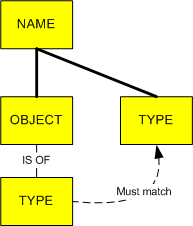
\includegraphics[scale=0.60]{img/static.png}
		\end{figure}
	
		\subsubsection{Example}	
			Here a java example: 
			\begin{lstlisting}[language=Java]
				int variable;
				variable = 10;
				variable = "ten";
			\end{lstlisting}
			It causes a compilation error:
			\begin{lstlisting}
				INSERIRE ERRORE DI COMPILAZIONE
			\end{lstlisting}
			
		\subsubsection{Advantages}
			\begin{itemize}
				\item  A large class of errors are caught in the early stage of development process;
				\item Static typing usually results in compiled code that executes more quickly because when the compiler knows the exact data types that are in use, it can produce optimized machine code.
			\end{itemize}
			
	\subsection{Dynamic type checking}
		Is the process of verifying the type safety of a program at runtime. It may cause a program to fail at runtime \textit{\textbf{(Wikipedia)}}.\\
		A language is dynamically typed if the type is associated with run-time values, and not named variables/fields/etc. This means that you as a programmer can write a little quicker because you do not have to specify types every time (unless using a statically-typed language with type inference) \textit{\textbf{(Stack Overflow)}}.\\
		In Dynamically typed languages, variables are bound to objects at run-time by means of assignment statements, and it is possible to bind the same variables to objects of different types during the execution of the program.
		Dynamic type checking typically results in less optimized code than static type checking. It also includes the possibility of run time type errors and forces run time checks to occur for every execution of the program (instead of just at compile-time) (\textbf{\textit{Schematic overview}}).\\
		
		\begin{figure}[h!]
			\centering
			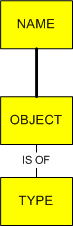
\includegraphics[scale=0.60]{img/dynamic.png}
		\end{figure}
	
		\subsubsection{Example}
			\begin{lstlisting}
				variable = 10
				variable = "ten"
			\end{lstlisting}
		
		\subsubsection{Advantages}
			\begin{itemize}
				\item Implementations of dynamically type-checked languages generally associate each run time object with a type tag (i.e., a reference to a type) containing its type information. This run-time type information (RTTI) can also be used to implement dynamic dispatch, late binding, down-casting, reflection, and similar features;
				\item The absence of a separate compilation step means that you don’t have to wait for the compiler to finish before you can test your code changes. This makes the debug cycle much shorter and less cumbersome.
			\end{itemize}
			
		CAPIRE SE SONO SOTTO CATEGORIE DI STATIC O DISTINZIONE PIU GENERALE 
	\subsection{Explicitly typed}
		Each variables is annotaded in source code with type's information. In this case the \textit{type check is simple but the language is more difficult} (from the programmers point of view).
			
	\subsection{Implicitly typed (inference)}
		The data types of source code are automatically detected. It is also rederred as \textbf{type inference}. The language \textit{is easier but the type check algorithm is far more complex}.
	\subsection{Strongly typed}
		A strongly-typed language is one in which variables are bound to specific data types, and will result in type errors if types do not match up as expected in the expression regardless of when type checking occurs. (\textbf{\textit{Schematic overview}})\\
		\subsubsection{Example}
			\begin{lstlisting}
				variable1 = 10
				variable2 = "ten"
				variable3 = variable1 + variable2
			\end{lstlisting}
	\subsection{Weakly typed} 
		A weakly-typed language on the other hand is a language in which variables are not bound to a specific data type; they still have a type, but type safety constraints are lower compared to strongly-typed languages.\\
			\begin{lstlisting}
				$temp = "ten"; 
				$temp = $temp + 10; // no error caused
				echo $temp;
			\end{lstlisting}
			
			
		
	
		\subsection{Example: type inference vs. dynamic typing}
			These two kind of typings could be confused. Here an example to clarify the differences:

			\begin{lstlisting}[language=Python]
				var1 = 10
				var2 = "astring"
				var3 = var1 + var2
			\end{lstlisting}
			
			\begin{enumerate}
				\item In \textbf{dynamically typed} language this code run without errors: at runtime the \textit{var1} is forced to be a string and the result is \textit{"10astring"};
				\item By the other side, in \textbf{inferred type language} the compiler \textit{throw an error}.
			\end{enumerate}
\newpage
\section{Python introduction}
	Python is a widely used general-purpose, high level programming language. It was initially designed by Guido van Rossum in 1991 and developed by Python Software Foundation. Python is an \textbf{interpreted}, \textbf{multi-paradigm} language. It support:
	\begin{itemize}
		\item Functional programming (non pure);
		\item Procedural programming;
		\item Objected oriented;
	\end{itemize} 
	Python uses \textbf{whitespace indentation}, rather than curly brackets or keywords, to delimit blocks. An increase in indentation comes after certain statements; a decrease in indentation signifies the end of the current block. \textit{Thus, the program's visual structure accurately represents the program's semantic structure}.\\
	Python uses \textbf{strict semantic}. \\
	It is usefull to recall the generale diffrences between \textbf{strict} and \textbf{lazy} evaluation:
	\begin{itemize}
		\item \textbf{Strict evaluation strategy}: the arguments of a function are fully evaluated to values before evaluating the function call, that is, before performing their replacement to formal parameters in the function body (\textbf{call by
		value}).
		\item \textbf{Non-strict or Lazy evaluation:} arguments are evaluated only if it is needed
		in the function body(\textbf{for instance, call by name}) .
	\end{itemize}
	Consequences concern expressiveness of the language (such as the ability of
	dealing with infinite lists) and the efficiency of the language implementation.
	\begin{lstlisting}
		def infiniteLoop(x):
			while True:
				print("do something with x")
			return x
		
		5 in [5, 10, infiniteLoop(5)]
	\end{lstlisting}
	In Python we never get \textit{true} beacause  he forced the evaluation of the function wich is an infinite loop.\\
	If we write the same code in \textbf{haskell} we get the \textit{true} value:
	\begin{lstlisting}
		elem 2 [2, 4, noreturn 5]
	\end{lstlisting}
	Typing:
	\begin{itemize}
		\item Python is \textbf{ dynamically typed},
		\item is a \textbf{strongly typed} language,
		\item use \textbf{duck typing}.
	\end{itemize}
\section{Python type checking}
	\subsection{Dynamic and strongly typed}
		Python is \textbf{dynamic}: objects have a type but it is determined at runtime. \\
		\textit{It rarely uses what it knows to limit variable usage.}
		
		\begin{lstlisting}
			if False:
				print(10+"ten") 
			else:
				print(10+10)
		\end{lstlisting}
		
		The first branch never execute, so the type checking ignore the type incongruency.\\
		Let's try to run:
		
		\begin{lstlisting}
			print(10+"ten")
		\end{lstlisting}
		
		Once executed the type check raise a type error:
		
		\begin{lstlisting}
			TypeError: unsupported operand type(s) for +: 'int' and 'str'
		\end{lstlisting}
		
		Another consequnce is that programmers are \textbf{free to bind the same names (variables) to different objects with a different type}. Then the following statements are perfectly legal:
		
		\begin{lstlisting}
			variable = 10
			variable = "ten"
		\end{lstlisting}
		
		So long as you only perform operations valid for the type the interpreter doesn't care what type they actually are. \\
		
		Python is also \textbf{strongly typed} as the interpreter keeps track of all variables types. In Python is not allowed to perform operations inappropriate to the type of the object: attempting to add numbers to strings will fail.
		
		One of the advantage of the \textbf{strongly typing} for the \textbf{dynamic} language is that \textit{you can trust what's going on:} if you do something wrong, your program will generate a type error telling you where you went wrong, and you don't have to memorize a lot of arcane type-conversion rules or try to debug a situation where your variables have been silently changed without your knowledge.
		
		
		There are some operations (methods, we will see later introducing duck typing) used even in case of type incongruence. \\
		The boolean equivalence is permitted in Python 2 and 3: 
		
		\begin{lstlisting}
		print("10" == 10)
		print("10" != 10)
		\end{lstlisting}
		
		Returning:
		
		\begin{lstlisting}
		False
		True
		\end{lstlisting}
		
		In Python 2 "\textit{grather than}" and \textit{"less than"} are permitted:
		
		\begin{lstlisting}
		print("10">10)
		print("10">=10)
		print("10"<10)
		print("10"<=10)
		\end{lstlisting}
		
		Returning:
		
		\begin{lstlisting}
		True
		True
		False
		False
		\end{lstlisting}
		
		Python 3 do not allowed to do "\textit{grather than}" and \textit{"less than"} controls.\\
		
	\subsection{Annotations}
		Annotations were introduced in Python 3.0 and are the main way to add type hints to the code. We can annotate both \textbf{function} and \textbf{variable}.
		
		\begin{lstlisting}
			import math
			
			pi: float = 3.142
			
			def circumference(radius: float) -> float:
				return 2 * math.pi * radius
		\end{lstlisting}
		
		Type hints and annotations do provide attributes that can be passed by 3rd party tools but du not add a real static typechecking in native Python so this should not effect the code performance significantly in the same way that comments don't.\\
		From PEP 484:\\
		\textit{ <...>Using type hints for performance optimizations is left as an exercise for the reader}.
		
		\begin{itemize}
			\item Type hints help document your code;
			\item Type hints improve IDEs and linters. They make it much easier to statically reason about your code. This in turn allows IDEs to offer better code completion and similar features. With the type annotation, PyCharm knows that text is a string, and can give specific suggestions based on this;
			\item Type hints take developer time and effort to add. Even though it probably pays off in spending less time debugging, you will spend more time entering code.
			\item Type hints introduce a slight penalty in start-up time. If you need to use the typing module the import time may be significant, especially in short scripts.	
		\end{itemize}
		
		
				
	\subsection{Duck typing}
	
		\subsubsection{Object oriented}
		
		The following code show how to declare a class, define a costructor for its parameters, define others methods and access to both.
		
		\begin{lstlisting}
			class Duck():
				#Constructor 
				def __init__(self, name, colour):
					self.name = name
					self.colour = colour
				
				def quack(self):
					return "Quaaack"
				
				def fly(self):
					return "The duck is flying"
			
			#Instantiate a istance of the Duck() class
			donald = Duck("Donald","white")
			
			#Access to fields and methods
			
			print(donald.name)
			print(donald.colour)
			
			print(donald.quack())
			print(donald.fly())
			
		\end{lstlisting}
		
		\begin{lstlisting}
			Donald
			white
			Quaaack
			The duck is flying
		\end{lstlisting}
		
		The first argument of every class method, including init, is always a reference to the current instance of the class. By convention, this argument is always named \textit{self}. In the init method, self refers to the newly created object; in other class methods, it refers to the instance whose method was called. \\
		The \textit{self} world is the equivalent of \textit{this} in \textbf{Java}. However Java do not requires to pass \textit{this} explicitly as a first parameter of a method, it could be used straight in the body of the method for its pourpouse.  	
		However self is not a reserved keyword in Python it’s just a strong convention. We could rewrite the previous class as follows:
		
		\begin{lstlisting}
			class Duck():
				#Constructor 
				def __init__(myself, name, colour):
					myself.name = name
					myself.colour = colour
			
				def quack(myself):
					return "Quaaack"
			
				def fly(myself):
					return "The duck is flying"
		\end{lstlisting}
		
		In Python is not possible to define multiple constructor for a class, still is possible to define a default value if one is not passed.
		
		\begin{lstlisting}
			class Parrot():
				def __init__(self, name = "Perry"):
				self.name = name
			
			bird1 = Parrot()
			bird2 = Parrot("Jack")
			
			print(bird1.name)
			print(bird2.name)
		\end{lstlisting}
		
		\begin{lstlisting}
			Perry
			Jack
		\end{lstlisting}
		
		
		\subsubsection{Main idea}
			
			Duck typing is a concept related to dynamic typing in an object oriented language. Is a feature in which the semantics of a class is determined by its ability to respond to some message (method or property) rather than being the extension of a class or an implementation of an interface. \\

			\textit{ If it looks like a duck, swims like a duck, and quacks like a duck, then it probably is a duck.}\\
			
			\begin{lstlisting}
				class Duck():
					def quack(self):
						return "Quaaack"
					def fly(self):
						return "The duck is flying"
				
				class Parrot():
					def quack(self):
						return "The parrot parrots a quack"
					def fly(self):
						return "The parrot is flying"
				
				class Man():
					def quack(self):
						return "The man parrots a quack too"
				
				v = [Duck(), Parrot(), Man()]
				
				for i in v:
				print(i.quack())
			\end{lstlisting}
			
			\textbf{The idea is that it doesn't actually matter what type my data is - just whether or not i can do what i want with it.}\\
			
			\begin{lstlisting}	
				for i in v:
					print(i.fly())
			\end{lstlisting}
			
			If we try to use the method \textit{fly()} over the entire collection of objects an error is raised at runtime:
			
			\begin{lstlisting}
				Traceback (most recent call last):
				File "/home/tommaso/git/ducktyping-tpl/code/ducklist.py", line 23, in <module>
				print(i.fly())
				AttributeError: Man instance has no attribute 'fly'
			\end{lstlisting}
			
			Lets see another example:
			
			\begin{lstlisting}
				class Car:
					def __init__(self, engine):
						self.engine = engine
					def run():
						self.engine.turn_on()			
			\end{lstlisting}
			
			This is a classical example of \textbf{dependency injection}. My class Car receives an instance of an engine and use it in the run method, where it calls the \textit{turn\_on} method. Note that my Car does not depends on any concrete implementation of engine. And I'm not importing any other type! Just using a dependency injected instance of something that responds to a \textit{turn\_on} message. I could say my class Car depends on an interface. But I did not have to declare it. \textbf{It is an "automatic interface"!}\\
			In a language \textbf{without} duck typing I'll probably have to declare an explicit interface named for example \textit{IEngine}, have the implementation (for example \textit{EngineV8}) and explicit define my Car parameter to be an implementation of IEngine.
			
			\begin{lstlisting}
				interface IEngine {
					void turnOn();
				}
				
				public class EngineV8 implements IEngine {
					public void turnOn() {
						// do something here
					}
				}
				
				public class Car {
					public Car(IEngine engine) {
						this.engine = engine;
				}
				
				public void run() {
					this.engine.turnOn();
			\end{lstlisting}
			
		Another intresting feature in Python, due to the duck typing, is the chance to add methods to the classes. First of all is important to say that in Python there is ad difference beetween:
		\begin{itemize}
			\item \textbf{Function};
			\item \textbf{Bound method}.
		\end{itemize} 
	
		Bound methods have been "bound" to an instance, and that instance will be passed as the first argument whenever the method is called.
		
		\begin{lstlisting}
			>>> def foo():
			...     print "foo"
			...
			>>> class A:
			...     def bar( self ):
			...         print "bar"
			...
			>>> a = A()
			>>> foo
			<function foo at 0x00A98D70>
			>>> a.bar
			<bound method A.bar of <__main__.A instance at 0x00A9BC88>>
			>>>
		\end{lstlisting}
		Callables that are attributes of a class (as opposed to an instance) are still unbound, though, so you can modify the class definition whenever you want.
		
	%	\begin{lstlisting}
	%		class Duck:
	%			pass
	%		
	%		def quack(myself, arg):
	%			myself.val = arg
	%			return myself.val
			
	%		donald = Duck()
	%		Duck.quack = quack
	%		print donald.quack("Quaaack!")
	%	\end{lstlisting}
		
		Recalling the previous example of calling a method on a list of object we have the following behaviour:
		
		\begin{lstlisting}
			donald = Duck()
			charlie = Parrot()
			john = Man("John")
			jack = Man("Jack")
			v = [donald, charlie, john, jack]
			
			def fly(self):
				return "Takes a plane"
			
			Man.fly = fly
			
			for i in v:
				print(i.fly())
		\end{lstlisting}
		
		The fly method was added to all the instances of Man class so that, when the fly method is called on the list there, are no errors at runtime. It is possible to add a method to a single istance of a class but we have a problem: the function is not automatically bound when it's attached directly to an istance. Let's modify a little the previous code adding a method to the instance "john" of the "Man" class.
		 
		\begin{lstlisting}
			def fly(self):
				return "Takes a plane"
			
			john.fly = fly
			
			for i in v:
				print(i.fly())
		\end{lstlisting}
		
		Running the code we have the following error:
		
		\begin{lstlisting}
			The duck is flying
			The parrot is flying
			Traceback (most recent call last):
			File "/home/tommaso/git/ducktyping-tpl/code/pokelist.py", line 33, in <module>
			print(i.fly())
			TypeError: fly() takes exactly 1 argument (0 given)
		\end{lstlisting}
		
		To bound the method properly to "john" we had to use the module \textit{types}:
		
		\begin{lstlisting}
			import types
			
			john.fly = types.MethodType(fly, john)
			
			for i in v:
				print(i.fly())
		\end{lstlisting}
		
		We still have an error but this time is caused by the istance "jack", proving that we added the method fly only to one istance of Man. 
		
		\begin{lstlisting}
			The duck is flying
			The parrot is flying
			Takes a plane
			Traceback (most recent call last):
			File "/home/tommaso/git/ducktyping-tpl/code/pokelist.py", line 35, in <module>
			print(i.fly())
			AttributeError: Man instance has no attribute 'fly'
		\end{lstlisting}
		
		
		
		
	
		
		






		
\end{document}